\section{提案手法}
既存手法の問題点として,ランダムな活性化関数の変更が挙げられる.探索後期において良いノードの出力の個体が生まれたとしても,例えば良いノードの活性化関数をlinear関数 $ f(x) = x $ からinverse関数 $ f(x) = -x $ に変更されてしまうと,ノードの出力は反転されてしまう.ネットワークの一部の構造化された部分の出力の大小は,同符号であれば出力層に大きな変化をもたらさないが,出力が0より大きいか小さいかは,ネットワークの出力は大きく変わることが知られている\cite{WANN}.\\
提案手法ではこれの問題を緩和するために,活性化関数の慎重な選択について言及する.2つの活性化関数の距離を計算し,距離が小さければ小さいほど変更先の活性化関数として選択されやすくなる.

\begin{figure}[h]
    \begin{center}
        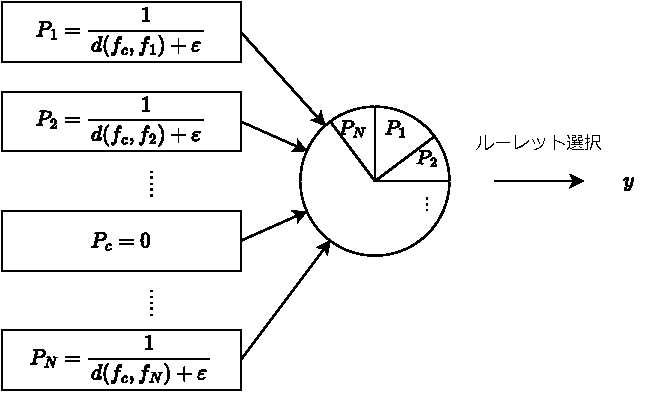
\includegraphics[scale=0.8]{img/exppropose.pdf}
        \caption{提案手法の概略図}
    \end{center}
\end{figure}

\begin{equation}
    P_{i} =  \begin{cases} \dfrac{1}{d(f_{c}, f_{i}) + \epsilon_{n} } \qquad (i \neq c) \\ 0 \qquad (i = c) \end{cases}\\
\end{equation}
\begin{equation}
    \epsilon_{n} = s * \epsilon_{n-1} \\
\end{equation}

\begin{table}[h]
    \caption{変数の説明}
    \centering
    \begin{tabular}{cl}
        \hline
        変数  & 意味 \\
        \hline \hline
        $P_{i}$               & $c$から$i$へ活性化関数IDが変更される見込み \\
        $d(f_{c}, f_{i})$     & 活性化関数が$c$と$i$の距離                 \\
        $f_{i}$               & IDが$i$の活性化関数                        \\
        $i$                   & 活性化関数ID                               \\
        $c$                   & 現在の活性化関数ID                         \\
        \hline
    \end{tabular}
\end{table}

まず現在の活性化関数 $ f_c $ と,すべての活性化関数との距離を計算する.この時の距離が小さいことは両者の関数が似ていることを意味し,距離の短い関数への変更は既存手法の問題点である出力の反転を防ぐ.距離が小さければ小さいほど選択されやすくするため,距離と $ \epsilon $ の和の逆数をルーレット選択の材料とする. $ \epsilon $ が大きくなると,ルーレット選択によって選ばれる確率はランダムに近くなる. $ \epsilon $ は探索初期においては,良いノードの出力を持つ個体が少ないことから,良い出力の個体を反転させてしまうデメリットより,悪い出力の個体を反転させるメリットの方が大きいと考え,探索初期の $ \epsilon $ は大きく,探索後期の $ \epsilon $ は小さく設定する.グラフは代表的な活性化関数4種,活性化関数同士の区間積分差を用いた活性化関数の変更として選択される確率を表した例である.\\

ここに図 \\

距離関数 $ d $ については,区間積分差と,個体の経験に基づく出力差を採用する.

\subsection{活性化関数同士の区間積分差}
式(7)は関数 $ f_a $ と $ f_b $ の範囲内の出力の差を意味している.

\begin{equation}
    d(f_{a}, f_{b}) = \int^{r}_{-r} (f_{a}(x) - f_{b}(x))^{2}
\end{equation}

\begin{table}[h]
    \caption{式(8)の変数の説明}
    \centering
    \begin{tabular}{cl}
        \hline
        変数  & 意味 \\
        \hline \hline
        $d(f_{a}, f_{b})$ & 活性化関数が$a$と$b$の距離                 \\
        $f_{i}$           & IDが$i$の活性化関数                        \\
        $r$               & 関数の考慮範囲                             \\
        \hline
    \end{tabular}
\end{table}

実際にネットワークにタスクを解かせる際,ノードへの入力は0付近である場合が多いので\cite{ノード入力}, $ -r $ から $ +r $ までの関数の区間積分によって距離を定義する.区間内の入力に対して出力の差が小さいことは,活性化関数を変更してもネットワークに大きな動作の変更をもたらさないことを意味し,局所的な解を優先的に探索する.番号が $ 1 $ から $ N $ と振られている活性化関数 $ f_n $ から $ f_N $ ,現在の活性化関数が $ f_c $, $ f_n $ と $ f_c $ の距離を $ d_n $ としたときの具体的なプログラムの実装は以下のようになる.

\begin{lstlisting}[caption=区間積分差のプログラム]
for n (1 to N)
    sum = 0
    for x (-r to +r)
        sum += (activate(x, n) - activate(x, c)) ^2
    d[n] = sum
\end{lstlisting}

ネットワークで使用する活性化関数にはそれぞれIDが1-based(1からナンバリングする方式)により割り振られており,1からNまでのそれぞれの活性化関数IDに対してその関数と変更前の関数との差の2乗を変数sumに加算していく.変数xをとても小さい数ずつ増やしていき,x範囲内の合計が最終的にsumに格納され,変更前の活性化関数の出力と活性化関数IDがnの関数の出力の差を2乗をd[n]に代入する.このように求めた $ d_n $ を式(6)に代入しルーレット選択により選ばれる見込み $ P_n $ を得る.
また, $ x $ を活性化関数の入力とした出力を求める関数 activate は後述する.

\subsection{個体の経験に基づく出力差}
式(7)は関数 $ f_a $ と $ f_b $ の個体が経験したノードの入力に対する差を意味している.
\begin{equation}
    d(f_{a}, f_{b}) = \sum_{m=1}^{M}(f_{a}(in_{m}) - f_{b}(in_{m}))^2
\end{equation}

\begin{table}[H]
    \caption{変数の説明}
    \centering
    \begin{tabular}{cl}
        \hline
        変数  & 意味 \\
        \hline \hline
        $d(f_{a}, f_{b})$ & 活性化関数が$a$と$b$の距離                 \\
        $f_{i}$           & IDが$i$の活性化関数                        \\
        $M$               & ミニバッチサイズと共有重みの積             \\
        $in_m$            & ミニバッチ $m$ 回目に経験したノードに入力される値 \\
        \hline
    \end{tabular}
\end{table}

区間積分差は範囲内のすべての領域を考慮し差を求めたのに対し,個体の経験に基づく出力差では,実際に個体がタスクを実行したときに経験した入力ノードの値を利用する.ネットワークの構造に変化はないので,入力ノードの値が分かれば,ネットワーク内の全てのノードの出力を特定することができ,ネットワークの変更にあたり指定した隠れ層のノードの出力を入力ノードから計算する.このとき指定したノードの活性化関数のみ変更し,この差を2乗を加算することで,個体が経験した入力に対する出力の差の小さい活性化関数を求めることができる.領域内を満遍なく考慮する手法よりも実際の入力ノードを利用することで出現確率の高いノード入力を大きく考慮することを期待する.ミニバッチには,同じ個体であれば異なる共有重みを使用していても利用する.

\begin{lstlisting}[caption=経験入力に基づく出力差のプログラム]
out(nodeID, actID, state, weight)
    preout = 0
    connect[] = synapses where the destination is nodeID
    node = Information of node where the ID is nodeID

    if(node[Type] == input)
        preout = state[nodeID]
    
    else
        for i (0 to connect)
            newnodeID = connect[source]
            newactID = activationID[connect[source]]
            val = out(newnodeID, newactID, state[x], weight)
            preout += val
    
    prein = preout * weight[m]
    output = activate(prein, actID)
    return output

weight = [-2.0, -1.0, -0.5, +0.5, +1.0, +2.0]
for n (1 to N)
    sum = 0
    for m (0 to 5)
        for x (0 to miniBatchSize)
            sum += (out(ID, n, m, state[x]) - out(ID, c, m, state[x])) ^2
    d[n] = sum
\end{lstlisting}

1からNまでの各活性化関数に対してノードの出力の差を求める.各共有重みに対してミニバッチのうちのひとつの入力ノード情報を利用する.state[x]には個体が経験した入力ノード情報が記憶されており,今回使用するタスクBipedalWalker-v2\cite{OpenAI}では,入力層のノードは24個なので要素数24の配列となる.ノードの出力を求める関数 out には,出力を求めたいノードID,活性化関数ID,入力ノード情報,共有重みの値を入力としている.関数 out に入力された nodeID が指すノードが入力層であれば入力ノードデータを返し,隠れ層であれば目的地が nodeID であるすべてのシナプスの 出発地になっているノードに対して出発地のノードIDを newnodeID ,出発地のノードの活性化関数IDを newactID として out を再帰的に実行する.シナプスの出発地を辿り続けるといつか必ず入力層となるため, val を必ず得ることができる.最初に呼び出した out に入力した nodeID に入力される値を今までの合計と共有重みの積から計算し,関数 activate に通すことで活性化関数の出力に対応する.最終的に関数 out は nodeID の出力を返し,異なる活性化関数 n と c の差の2乗を sum に加算していく.区間積分の手法と同じく n と c の差は d[n] に代入される.ソースコード2の out(ID, n, m, state[x]) は式(9)の $ f_{a}(in_{m}) $ と同等の意味を持つ. $ x $ を活性化関数の入力とした出力を求める関数 activate は後述する.

\subsection{用いる活性化関数}
今回用いる活性化関数には,1-basedにナンバリングされ,以下の10種類を用いる.また関数への入力 $ x $ に対応する出力 $ y $ を示した数学的表現,pythonで実装した入力 x に対応する value を示す.

\begin{table}[H]
    \caption{用いる活性化関数とその式}
    \centering
    \begin{tabular}{clll}
        \hline
        ID & 関数名 & 数学的表現 & プログラム上での表現 \\
        \hline \hline
        1 & Linear & $ y = x $ & value = x \\
        2 & Step & $ y = \begin{cases}
            1.0 & (x > 0.0) \\
            0.0 & (x \leq 0)
            \end{cases} $ & \texttt{value = 1.0*(x>0.0)} \\
        3 & Sine & $ y = \sin(\pi x) $ & value = np.sin(np.pi*x) \\
        4 & Gaussian & $ y = e^{-\frac{x^2}{2}} $ & value = np.exp(-np.multiply(x, x) / 2.0) \\
        5 & Hyperbolic Tangent & $ y = \frac{e^{x} - e^{-x}}{e^{x} + e^{-x}} $ & value = np.tanh(x) \\
        6 & Sigmoid & $ y = \frac{\tanh\left(\frac{x}{2}\right) + 1}{2} $ & value = (np.tanh(x/2.0) + 1.0)/2.0 \\
        7 & Inverse & $ y = -x $ & value = -x \\
        8 &Absolute & $ y = |x| $ & value = abs(x) \\
        9 & Relu & $ y = 
        \begin{cases}
        x & (x > 0)\\
        0 & (x \leq 0)
        \end{cases} $ & value = np.maximum(0, x) \\
        10 & Cosine & $ y = \cos(\pi x) $ & value = np.cos(np.pi*x) \\
        \hline
    \end{tabular}
\end{table}

上で使用した activate 関数は,入力値と活性化関数IDとし,表に従いvalueを出力する.

\subsection{距離関数の妥当性}
提案手法では,活性化関数同士の出力の差の大きさを距離関数として表現している. \\
実数の組から実数への写像を実現する関数 $ d: \mathbb{R} \times \mathbb{R} \rightarrow \mathbb{R} $ が距離関数であるとは, $ x, y, z $ を $ \mathbb{R} $ の任意の元として,以下の条件が満たされていることを言う\cite{距離関数}.

\begin{table}[H]
    \caption{距離関数の性質}
    \centering
    \begin{tabular}{cl}
        \hline
        性質  & 定義 \\
        \hline \hline
        非負性     & $ d(x, y) \geq 0 $ \\
        同一律     & $ d(x, y) = 0 \Leftrightarrow x = y $ \\
        対称律     & $ d(x, y) = d(y, x) $ \\
        三角不等式 & $ d(x, y) \leq d(x, z) + d(z, y) $ \\
        \hline
    \end{tabular}
\end{table}

同一律については,$ d(x, x) = 0 $ とは違う意味を示していることに注意する. $ x $ と $ x $ の距離は当然0であるが, $ x $ と $ y $ が同一でない限り距離が0にはならないことを示している.つまり $ x $ と $ y $ が別のものを指しているのに関わらず距離が0になった場合,その関数dは距離関数としての性質を満たしていないことになる.これらの証明をするにあたって,2つの提案手法について確認する.式(8)と式(9)はいずれも一定の数の要素を持つ配列の,各要素同士の差を2乗したものの総和ととれる.各要素の値はどのようなものであっても距離関数を満たすため,ここでは以下のようにし証明を簡略化する.

\begin{equation}
    d(a, b) = \sum_{i=o}^{N-1}(a[i] - b[i])^2
\end{equation}

ここで $ f_{a}(x) $ や $ f_{a}(in_{m}) $ を $ a[i] $ とすることは,どのような実数に対しても関数が距離関数の性質を持つことから,そのうちの一例である $ f_{a}(x) $ や $ f_{a}(in_{m}) $ も例外でなく距離関数の性質を持つと導くことができる.以下は同じ要素数の配列に任意の実数を代入したときに式(10)が距離関数として成立しているかの証明になる.

\begin{enumerate}
    \item 非負性 \\
    任意の実数 $ a[i] $ と $ b[i] $ の差は必ず実数となり,実数の2乗は必ず0以上の実数になる.有限の個数の0以上の実数の和もまた必ず0以上の実数となることから,式(10)は非負正を満たす.

    \item 同一律 \\
    $ (a[i] - b[i])^2 $ が必ず0以上の実数となり,0になるのは $ a[i] $ と $ b[i] $ の値が等しい場合のみであることから,関数 $ d $ が0になるのは,すべての要素に対して $ a[i] $ と $ b[i] $ が等しい必要がある.これは全ての要素について $ a[i] = b[i] $ であることを意味し,同一率を満たす.

    \item 対称律 \\
    $ x^2 = (-x)^2 $ であることから,$ (a[i] - b[i])^2 = (b[i] - a[i])^2 $ と言える.その総和もまた等しいため,関数dは対称律を満たす.

    \item 三角不等式 \\
    三角不等式の証明にはシュワルツの公式

    \begin{equation}
        \sum_{k=1}^n p_iq_i \leq \sqrt{\sum_{k=1}^n p_i^2 + \sum_{k=1}^n q_i^2}
    \end{equation}

    を用いる.まず $ a $ の各要素を $ a_0, a_1, a_2, ..., a_m $ とし,これと同じく $ b, c $ についても表す.次に

    \begin{equation}
        p_i = , q_i = b_i - c_i
    \end{equation}

    とし,これより

    \begin{equation}
        p_i + q_i = b_i - a_i
    \end{equation}

    を得る.対称律,式(11),式(12),式(13)を用いると

    \begin{eqnarray}
        \{ d(a, b) \}^2 &=& \{ d(b, a) \}^2 \notag \\
        &=& \{ \sum_{i=0}^{N-1}(b_i - a_i)^2 \}^2 \notag \\
        &=& \{ \sum_{i=0}^{N-1}(p_i + q_i)^2 \}^2 \notag \\
        &=& \{ \sum_{i=0}^{N-1}(p_i^2 + 2p_iq_i + q_i^2) \}^2 \notag \\
        &=& \{ \sum_{i=0}^{N-1}p_i^2 + \sum_{i=0}^{N-1}2p_iq_i + \sum_{i=0}^{N-1}q_i^2 \}^2 \notag \\
        &\leq& \{ \sum_{i=0}^{N-1}p_i^2 + 2\sqrt{\sum_{i=o}^{N-1}p_i^2\sum_{i=0}^{N-1}q_i^2} + \sum_{i=0}^{N-1}q_i^2 \}^2 \notag \\
        &=& \{ (\sqrt{\sum_{i=0}^{N-1}p_i^2} + \sqrt{\sum_{i=0}^{N-1}q_i^2})^2 \}^2 \notag \\
        &=& \{ \sum_{i=0}^{N-1}p_i^2 + \sum_{i=0}^{N-1}q_i^2 \}^2 \notag \\
        &=& \{ \sum_{i=0}^{N-1}(c_i - a_i)^2 + \sum_{i=0}^{N-1}(b_i - c_i)^2 \}^2 \notag \\
        &=& \{ d(a, c) + d(c, b) \}^2 \notag \\
        d(a, b) &\leq& d(a, c) + d(c, b)
    \end{eqnarray}
\end{enumerate}

より三角不等式を満たす.\\

これらの証明は,いずれもa[i]の要素の集合が実数集合のうちの一部であることに注意する.例えば式(8)では $ -r $ から $ r $ までの限られた範囲に過ぎない.式(9)では経験した入力ノードの組み合わせ,さらにそのミニバッチサイズ分のデータに対しての距離を計算しているに過ぎない.Linear関数とRelu関数は $ x $ が0以上のみの入力を考慮した場合距離が0になってしまうが,実際これらの活性化関数は負の領域では全く異なる性質を持つ.しかしこの式は,ネットワークが多くの場面で経験する値を想定して入力として扱っている.0より大きく離れた値はノードの入力にはめったに使われなかったり,経験した入力ノードの値から大きく外れたものもあまり考慮する必要がないという考え,今回の提案手法を採用した.